\documentclass[12pt,epsf,psfig,graphics]{article}             
\textwidth = 6.5in
\textheight = 9.05in
\topmargin 0.0in
\oddsidemargin 0.0in
\evensidemargin 0.0in

% set it so that subsubsections have numbers and they
% are displayed in the TOC (maybe hard to read, might want to disable)

\usepackage[T1]{fontenc}
\usepackage{mathptmx}

\usepackage{graphics}

\setcounter{secnumdepth}{3}
\setcounter{tocdepth}{3}

% define widow protection 
        
\def\widow#1{\vskip #1\vbadness10000\penalty-200\vskip-#1}

% define a little section heading that doesn't go with any number

\def\littlesection#1{
\widow{2cm}
\vskip 0.5cm
\noindent{\bf #1}
\vskip 0.1cm
\noindent
}

% A paraphrase mode that makes it easy to see the stuff that shouldn't
% stay in for the final proposal

\newdimen\tmpdim
\long\def\paraphrase#1{{\parskip=0pt\hfil\break
\tmpdim=\hsize\advance\tmpdim by -15pt\noindent%
\hbox to \hsize
{\vrule\hskip 3pt\vrule\hfil\hbox to \tmpdim{\vbox{\hsize=\tmpdim
\def\par{\leavevmode\endgraf}
\obeyspaces \obeylines 
\let\par=\endgraf
\bf #1}}}}}

\renewcommand{\baselinestretch}{1.2}    % must go before the begin of doc
\newtheorem{principle}{Principle}
\newtheorem{definition}{Definition}
\newtheorem{define}{Definition}
% go with the way that CC sets the margins

\usepackage{listings}

\usepackage{color}

\definecolor{javared}{rgb}{0.6,0,0} % for strings
\definecolor{javagreen}{rgb}{0.25,0.5,0.35} % comments
\definecolor{javapurple}{rgb}{0.5,0,0.35} % keywords
\definecolor{javadocblue}{rgb}{0.25,0.35,0.75} % javadoc

\begin{document}

\lstset{language=Java,
basicstyle=\ttfamily,
keywordstyle=\color{javapurple}\bfseries,
stringstyle=\color{javared},
commentstyle=\color{javagreen},
morecomment=[s][\color{javadocblue}]{/**}{*/},
%numbers=left,
numberstyle=\scriptsize\color{black},
stepnumber=1,
numbersep=7pt,
tabsize=4,
showspaces=false,
showstringspaces=false}

% handle widows appropriately
\def\widow#1{\vskip #1\vbadness10000\penalty-200\vskip-#1}

\begin{center}

CMPSC 440: Operating Systems\\
Examination One\\
%Saturday December 11, 2004 \\

\end{center}

\noindent
Answer the five questions that are listed on the following pages.  You must provide answers to these questions on a
separate sheet of paper.  Please develop responses that clearly express your ideas in the most succinct manner possible.
You are not permitted to complete this examination in conjunction with any of your classmates.  Furthermore, you cannot
consult any outside references during this examination.  If you have questions concerning the following problems, then
please visit my office during the examination period.  If you leave the classroom to take the exam, then you are
responsible for checking the white board for status updates.

%\mbox{} \newline
%\mbox{} \newline

\begin{enumerate}
  
\item ({\bf 10 Points}) The operating system is a resource manager for the hardware provided by the computer.  Answer
  the following questions about the management of computer hardware.

  \begin{enumerate}
          
  \item ({\bf 2 Points}) The computer contains resources that must be shared through either time or space multiplexing.
    What are these two types of multiplexing? What is an example of a resource that can be shared with each of these
    methods?
   
  \item ({\bf 5 Points}) A typical memory hierarchy contains five levels.  Arrange the levels of the memory hierarchy so
    that the fastest and smallest type of memory is at the top of your diagram and the slowest and largest is at the
    bottom.
  
  \item ({\bf 3 Points}) There are three canonical strategies for performing input and output with the
    kernel and device drivers.  What are these strategies? What are their trade-offs?

  \end{enumerate}
        
\newpage

\begin{figure}[t]
  \centering
  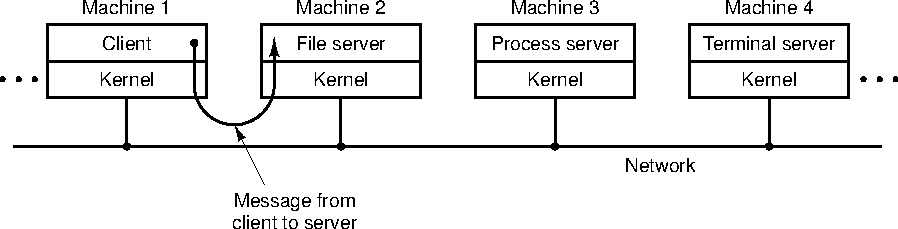
\includegraphics{fig1-27}
  \caption{Client-Server Communication Involving the Client, a Server, and the Kernel.}
  \label{fig:clientserver}
\end{figure}

\item ({\bf 10 Points}) There are many basic concepts that under gird the fundamentals of operating systems.  Answer the
  following questions about basic operating systems concepts.

  \begin{enumerate}
          
  \item ({\bf 4 Points}) A real-time operating system must schedule tasks to guarantee that a specified deadline will be
    met.  Draw a graph with a horizontal axis called ``time'', a vertical axis called ``utility'', and a vertical line
    at point $D$ on the horizontal axis.  Now, please draw a utility curve that represents the challenge associated with
    scheduling in a real-time operating system. Why did you draw this curve the way that you did?

  \item ({\bf 3 Points}) The shell of an operating system allows for the composition of processes using the pipe and
    filter architecture.  In the following code segment, what is the pipe? What is the filter? Why is this a good mode
    of interaction with the operating system?

    \begin{quote}
      {\tt cat file1 file2 file3 | sort > /dev/lp \&}
    \end{quote}

  \item ({\bf 3 Points}) Figure~\ref{fig:clientserver} furnishes an example of a client communicating with the server
    with the support of the operating system kernel. Please outline all of the steps that must take place to support the
    communication between ``Machine 1'' and ``Machine 2''. 

  \end{enumerate}

  \newpage

\item ({\bf 10 Points}) Most, if not all, operating systems provide a kernel and many support virtualization. Answer the
  following questions about kernels and virtualization methods.

  \begin{enumerate}

    \item ({\bf 2 Points}) Most virtualization techniques distinguish between the guest operating system and the host
      operating system.  What is the meaning of these two terms? 

    \item ({\bf 3 Points}) How does the Java virtual machine support the standard of write-once run-anywhere? Your
      response to this question should use a properly labeled diagram.

    \item ({\bf 3 Points}) There are three representative types of operating systems kernels: microkernels, exokernels,
      and monolithic kernels. Using a properly labeled diagram for each definition, explain these types of kernels. What
      are their strengths and weaknesses?

    \item ({\bf 2 Points}) When implementing the process scheduler for the kernel, it is normally useful to separate
      policy and mechanism.  What does this maxim mean? \mbox{Why is it important}?


  \end{enumerate}

  \newpage

  \begin{figure}[t]
    \centering
    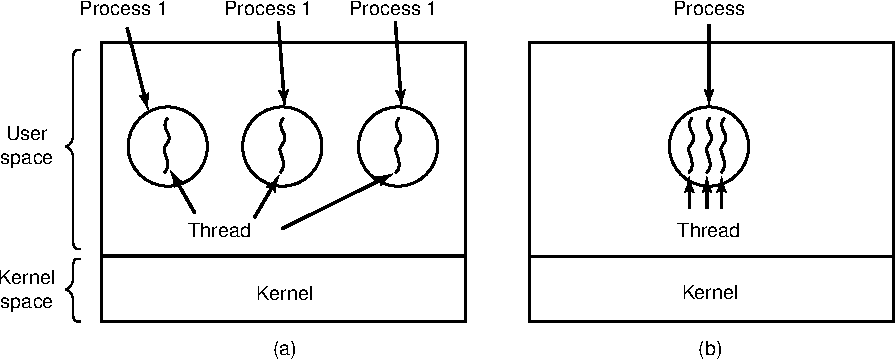
\includegraphics{fig2-11}
    \caption{Different Configurations of Processes and Threads.}
    \label{fig:pandt}
  \end{figure}


\end{enumerate}

\end{document}

